\documentclass{report}
\usepackage{bbold}
\usepackage{amsfonts}
\usepackage{graphicx}
\graphicspath{./Images/}
\usepackage{amssymb}
\usepackage{physics}
\usepackage{tensor}
\usepackage{hyperref}
\usepackage{amsmath}
\hypersetup{
  colorlinks=true,
  linkcolor=blue,
  filecolor=magenta,      
  urlcolor=cyan,
  pdftitle={Notes},
  pdfpagemode=FullScreen,
}

\author{Jay Rashamiya}
\begin{document}

\begin{titlepage}
  \begin{center}
    \line(1,0){300}\\
    \huge{\bfseries Tricks and Techniques}\\
    \line(1,0){300}\\
    \textsc{\LARGE Jay Rashamiya}\\
    \vspace{5cm}
  \end{center}

  \noindent \textsc{\large I knew a lot of things. Over time, I forgot many things. Now, I only know a few things. Therefore I took the wise decision of noting stuff down. To start, I try to summarize the most elementary things I knew, and the hope is that I'll keep on adding new things that I learn. For now, it's almost all the undergrad stuff which I am trying to summarize as quickly as possible.}
\end{titlepage}

\tableofcontents


\chapter{Feel of the scale : Read twice everyday}

I always disliked remembering numerical values. I was satisfied with the qualitative nature of things. Fortunately, I found a very old book (Newtonian Mechanics by AP French) which made me realise the kind of grave mistake I was doing. If you don't wish to read him, the summary is : A physicist must know the rough scale of things.\\

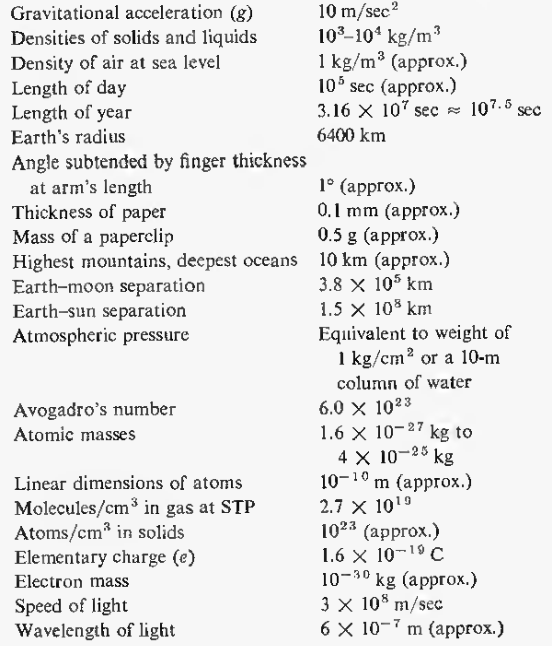
\includegraphics[width= 12cm, height=10cm]{./Images/Scales.png}


\chapter{Magic of Infinitesimals}
\section{Continuity}
\subsection{Any mid value}
\textbf{Statement:} If function $f(x)$ is continuous in the interval $[a,b]$ with $f(a) = A$ and $f(b) = B$, then every value in the interval $[A,B]$ is achieved. Namely, $\forall N \in [A,B], \exists \xi \in [a,b]$ such that $f(\xi) = N$ \\

\noindent\textbf{Proof:} Not required.

\subsection{Max and Min value}
\textbf{Statement:} If the function is continuous in a closed interval than it has a largest and a smallest value for atleast one $x$ in that interval. (Other way of saying that it doesn't become infinite). \\

\noindent\textbf{Use:} In rolle's theorem, for the existence of highest value.

\section{Differentiability}
\subsection{Rolle's Theorem}
\textbf{Statement :} If the function is differentiable in the interval $[a,b]$ and $f(a) = f(b)$, $\exists$ $\xi$ $\in$ $(a,b)$ such that $f'(\xi) = 0$. \\

\noindent\textbf{Proof :} Use sign change/existence argument at maximum.\\

\noindent\textbf{Use :} Finding remainder term in taylor series. Proving L'Hopital rule and various other places where we construct a new function on which we can apply Rolle to prove certain thing about a given function.\\

\subsection{Mean Value theorem}
\textbf{Statemnt :} For a differentiable function in a given interval $[a,b]$, $\exists$ $\xi$ $\in$ $(a,b)$ such that $f'(\xi) = \frac{f(b)-f(a)}{b-a}$ \\

\noindent\textbf{Proof :} Using rolle's theorem.\\

\noindent\textbf{Use :} $f(b) = f(a) + (b-a) f'(a+\theta (b-a))$, $\theta \in [0,1]$.

\subsection{Taylor series}
A function which can be differentiated arbitary number of times can always be expanded as \\\

\begin{equation}
f(b) = f(a) + (b-a)f'(a) + \frac{(b-a)^2}{2!}f''(a) + \dots + \frac{(b-a)^n}{n!}f^{(n)}(a) + R_n
\end{equation}
The remainder term can be beautifully calculated using rolle's theorem as 

$$R_n = \frac{(b-a)^{n+1}}{(n+1)!} f^{(n+1)}(\xi)$$

\noindent Clearly, this tends to zero as n tends to infinity if the derivative is bounded (which is, because we assumed it exists). A clever trick for finding out taylor series for indefinite integrals is to find the taylor series of integrand and integrate them.

\section{Infinitesimals}
Summing up (infinite times), or dividing is same as summing up (infinite times) or divding only the principal part.\\

\noindent Three properties are important for geometric visualization of calculus:\\

\noindent \textbf{Property 1 :} Any general arc differes from its chord by an infinitestimal of a higher order. Using this, we can imainge arcs as chords (and same extension in higher dimensions, curved surface as planes). We can find the curve length by ignorigng this higher order infinitesimal differnce between arc and chord because infinite sum of infinitesimals is same as infinite sum of their principal parts.\\

\noindent \textbf{Property 2 :} Perpendicular distance from one end of the infintestimal arc to the tangent at the other end  is an infitesimal of higher order than arc, however the length of the tangent from the foot of prependicular to the point of tangency is of the same order. You can prove this by using maclaurine series in transformed coordinates or by simple geometric construction.\\

\noindent \textbf{Property 3 :} Same trigonometric laws are obeyed. This is because the chord becomes tangent to the arc as their length approaches zero. The rules of chord extend to the arcs.

\section{Differentials}

Note that for an independent variable $d^2x = 0$, not otherwise. For independent variable $x$, differential $dx$ is same as infinitesimal increment $\Delta x$ to x. For dependent variable $y$, the differential $dy$ is the principal part of the infinitesimal change $\Delta y$ in $y$. The rules for differentials can easily be derived.

$$\lim_{\Delta x\to 0} \frac{\Delta y}{\Delta x} = f'(x)$$
$$\Delta y = f'(x)\Delta x + \epsilon\Delta x$$
$$dy = f'(x)dx$$

\noindent Knowing usual rules for differnetials, we can use them as algebraic quantities, no need to think of differential operators.\\

\noindent Note the difference between the context of the symbol $\frac{d^2 y}{dx^2}$. Which has context independent meaning only when x is independent variable.\\

\noindent\textbf{Implicit Function Theorem :} If $F(x,y)=0$ and $|F_x| < \infty$ with $F_y\neq 0$, then $y(x)$ exists and is differentiable. Can be easily extended to higher dimensions and/or involving more than one function using jacobians.

\chapter{Sequences}
I list all the theorems which you can prove in order and digest.\\

\noindent\textbf{Defn :} A sequence $(x_n)$ is said to convere to $x$ if $\forall \epsilon > 0$, $\exists N\in \mathbb{N}$ such that $|x_n - x| < \epsilon, \forall n > N.$ \\

\noindent \textbf{Theorem 1 :} If sequence $(x_n)$ converges, it has a unique limit point.\\

\noindent \textbf{Thorem 2 :} If sequence $(x_n)$ converges, it is bounded. (Bounded : $\exists M \in \mathbb{R}$ such that $\forall n,  |x_n| < M$).\\

\noindent \textbf{Theorem 3 :} If a \textbf{monotone} sequence $(x_n)$ is bounded, then it converges. The limit is $sup\{x_n : n \in \mathbb{N}\}$ \\

\noindent \textbf{Theorem 4 :} Every subsequence of a convergent sequence converges to the limit of sequence.\\

\noindent \textbf{Theorem 5 :} Every sequence has a monotone subsequence.\\

\noindent \textbf{Theorem 6 :} (Bolzano) Every bounded sequence has a convergent subsequence. (Just a consequence of prev theorem)\\

\noindent \textbf{Defn :} Limsup/ Liminf of sequence $(a_n)$ are defined by 

$$\limsup_{n\to\infty} a_n = \lim_{n\to\infty}sup(\{a_k : k>=n\})$$ 
$$\liminf_{n\to\infty} a_n = \lim_{n\to\infty}inf(\{a_k : k>=n\})$$ \\

\noindent \textbf{Thoerem 7 :} limsup/liminf of a bounded sequence always exists.\\

\noindent \textbf{Theorem 7 :} Let $(x_n)$ be a bounded sequence. Then $\exists$ subsequences $(x_{n_k})$ and $(x_{m_k})$ s.t.
$$\lim_{n\to\infty}x_{n_k} = \limsup x_n$$
$$\lim_{n\to\infty}x_{n_k} = \liminf x_n$$



\noindent \textbf{Theorem 8 :} If every convergent subsequence of $(x_n)$ has the same limit $x$, then $(x_n)$ converges to $x$.\\

\noindent \textbf{Cauchy Sequence :} A sequence $(x_n)$ is cauchy sequence, if $\forall \epsilon > 0, \exists N \in \mathbb{N}$ such that $|x_n - x_m| < \epsilon , \forall m,n> N$\\

\noindent \textbf{Theorem 9 :} \textbf{A sequence $(x_n)$ converges iff it's a Cauchy sequence.}\\

This theorem is great, because we don't need to know $x$ beforehand to check if the sequence converges to $x$. All we care about is the behaviour of the sequence. Namely, terms get closer and closer. Also useful for deriving various tricks to check convergence of a series.




\chapter{Series}
Same presentation as chapter 2.\\

\noindent \textbf{Defn : }If $(a_n)$ is a a sequence of real numbers then the series $\sum_{n=1}^{\infty}a_n$  converges to $S \in \mathbb{R}$ if the seuqnece $(S_n)$ of partial sum converges to $S$.\\

\noindent \textbf{Trick : } For geometric and telescopic series, you can find explicit formula for $n^{th}$ term of the sequence $(s_n)$.\\

\noindent \textbf{Theorem 1 :} A series $\Sigma a_n$ of positive term converges iff its partial sums are bounded.\\

\noindent \textbf{Theorem 2 :} (Cauchy Condition) The series $\Sigma a_n$ converges iff $\forall \epsilon > 0, \exists N \in \mathbb{N}$ such that $|S_n - S_m| < \epsilon, \forall n > m > N$\\

\noindent \textbf{Defn :} Series $\Sigma a_n$ converges absolutely if $\Sigma |a_n|$ converges. It converges conditionally if $\Sigma a_n$ converges but $\Sigma |a_n|$ diverges.\\

\noindent \textbf{Theorem 4 :} Absolutely convergent series $\Sigma a_n$ converges. Moreover, $\Sigma a_n$ converges absolutely, iff series $\Sigma a_n^{+}$ and $\Sigma a_n^{-}$ converges.\\

Follwoing tests can all be proved simply, using cauchy criterion.\\

\noindent \textbf{Test for divergence :}  If series $\Sigma a_n$ converges, then $\lim_{n\to\infty} a_n = 0$ \\

\noindent \textbf{Comparision test :} If $b_n\ge0, \Sigma b_n$ converges, then $\Sigma a_n$ converges absolutely if $|a_n| \le b_n$\\

\noindent \textbf{Ratio test :} If $(a_n)$ is a sequence of nonzero real numbers, let 
$$ r = \lim_{n\to\infty}\Bigl|\frac{a_{n+1}}{a_n}\Bigr|$$
\noindent Series $\Sigma a_n$ converges absolutely if $0\le r<1$, diverges if $1<r\le \infty$\\

\noindent \textbf{Root test :} For $(a_n)$
$$ r = \lim_{n\to\infty} sup|a_n|^{\frac{1}{n}}$$
\noindent The series converges absolutely if $0\le r<1$ and diverges if $1<r<\infty$.\\

\noindent\textbf{Alternating series test :} If $(a_n)$ is a decreasing sequence of nonnegative real numbers, such that $lim_{n\to\infty}a_n=0$, then the alternating series $\Sigma (-1)^{n+1}a_n$ converges.\\

\noindent\textbf{Limit Comparisiont test :} If $\Sigma a_n$ and $\Sigma b_n$ are two seires and 

$$ r:= \lim_{n\to\infty}\big(a_n/b_n\big) $$

\noindent If $r=0$ : If $\Sigma b_n$ converges, then $\Sigma a_n$ converges.\\
\noindent If $r=\infty$ : If $\Sigma b_n$ diverges, then $\Sigma a_n$ diverges.\\
\noindent IF $r$ is finite, either both converge or both diverge.\\

\noindent\textbf{Theorem 4 :} Every rearrangement of an absolutely convergent series converges to the same sum.\\

\section{Power series :}

There's only one power series for a given funcion (Coefficients are obviously uniquely defined by differentiation).

\begin{itemize}

  \item If a power series converges for some $x=x_1$, it converges absolutely and uniformly for all $|x_2| < |x_1|$. This can be proven using comparision test.\\

    Follwowing are the conseqences of uniform convergence :

    \begin{enumerate}
      \item The function defined by power series is continuous inside the region of convergence. 

      \item The power series can be integrated term by term in the region of convergence.

      \item The power series can be differentiated term by term. This is a more restrictive condition : the continuity of all individual derivatives as well as  the uniform convergence of the series formed by derviative is required.

    \end{enumerate}

  \item On the boundary of region of convergence, there is atleast one singularity.

\end{itemize}

\chapter{Complex Variables}

\begin{itemize}

  \item Cauchy reimann conditions for analyticity are sufficient when first order derivatives are also continuous. Analyticity is defined as differentiability in a region. 

  \item As an example $|z|^2$ is differentiable at $z=0$ but not analytic anywhere.

  \item The corresponding real functions of analytic function are harmonic and the conjugate functions form an orthogonal family. Moving along one would give maximum change in the other. The mapping is conformal at points when $f'(z) \neq 0$ or $f'(z) \neq \infty$.

\end{itemize}

\section{Cauchy's Theorem and Integral Formula} If $f(z)$ is analytic in a simply connected region and $C$ is a closed contour in that region then

\begin{gather}
\oint_{C}f(z)dz = 0\\
\frac{1}{2\pi i}\oint_{C}\frac{f(z)}{z-z_0}dz = f(z_0)
\end{gather}

\begin{enumerate}
  \item Taylor and laurent series are simple consequence of this.
  \item Residue is very important for performing various integrals and summing series(as that is the only term that will remain after integration). 
  \item Apart from poles and essential singularity, branch points are also a type of singularity.
  \item for $z^\frac{1}{2}$, the branch point is at $z=0$, order is defined as the number of paths around that point to return to same value. In this case it's $2$.
\end{enumerate}


\section{Analytic Continuation}
In real analysis, a function defined on a given range can be smoothly extended to outer regions in many ways. There's only a unique way to do so for analytic functions. This great property makes complex analysis almost GODLY.\\

\noindent If two analytic functions coincide in any region, or on any finite line segment, they are the same function.


\chapter{Differential Equations}

\section{A notational devil}

You have seen the notation 

$$\frac{\partial f}{\partial y^i}  = \frac{\partial f}{\partial x^j}\frac{\partial x^j}{\partial y^i}$$

\noindent Here, $f$ is a function which can have different form as expressed in $y$ coordinates. The notation $\frac{\partial f}{\partial y^i}$ really means that we are differentiating the function $f$ expressed in $y$ coordinates with respect to the $i^{\mathrm{th}}$ entry. In a more precise form it is seen as 

$$\frac{\partial f}{\partial y^i} := \partial_i(f\circ y^{-1})$$

\noindent I won't even mention ODE's with constant coefficients.
\section{First Order ODE}

\begin{itemize}
  \item One can always find integrating factor for first order ODE in principle. In practice, we only know direct formula for \textbf{linear} first order ODE. This also means that every differential constraint (in two dimensions) is holonomic.

  \item List of famous non-linear first order equations that can be solved

    \begin{enumerate}
      \item Bernoulli equation
        $$\frac{dy}{dx} + P(x)y = Q(x)y^n$$
      \item Clairaut's equation
        $$y = x\frac{dy}{dx} + f\left(\frac{dy}{dx}\right)$$
      \item D'Alembert's equation
        $$y = xf\left(\frac{dy}{dx}\right) + g\left(\frac{dy}{dx}\right)$$
    \end{enumerate}

\end{itemize}

\section{Second Order Linear ODE}
Most important differential equations arising in physics are almost always second order and linear (ordinary or partial). Let's consider only the homogenous part right now.
$$y'' + P(x)y' + Q(x) = 0$$

\noindent \textbf{Ordinary Point :} $x_0$ for which $P(x_0)$ and $Q(x_0)$ are finite.\\

\noindent \textbf{Regular Singular Point :} Singular $x_0$ for which $(x-x_0)P(x)$ and $(x-x_0)^2 Q(x)$ remain finite.\\

\noindent \textbf{Irregular Singular Point :} Singular $x_0$ for which one of $(x-x_0)P(x)$ or $(x-x_0)^2 Q(x)$ diverge.\\

\begin{itemize}
  \item The only trick we know is Frobenius! Always check if the final solution converges. You have to expand about a clever point. Expanding about essential singularity won't work.\\

  \item Expressing ODE as $L(x)y(x) = 0$. If $L(x) = L(-x)$, then if $y(x)$ is a solution, so is $y(-x)$. So you can express general solution as a linear combination of odd and even.
\end{itemize}

\noindent \textbf{Wronskian :} To test for linear independence of functions, we obtain $n$ equations by differentiating the relation 

$$\sum_{i=0}^{n}a_i \phi_i (x) = 0$$

\noindent This is the origin of Wronskian! Also used in some ninja-technical way to find particular solution for inhomogenous linear equation.

\subsection{Sturm-Liouville Theory}

In physics, we don't really require general solutions. We require solutions with specific boundary conditions. Specific boundary conditions impose conditions on the parameters of the equation. For instance, for a string clamped at $x=0$ and $x=l$, in the differential equation $\frac{d^2\psi}{dx^2} + k^2\psi(x) = 0$ , $k$ will have certain restrictions as you know. Here, $k^2$ is the eigenvalue.\\

\noindent Charecterization of general features of eigenproblems arising \textbf{from linear second-order differential equations} is known as Strum-Liouville theory.\\

\noindent Consider $\mathcal{L}\psi(x) = \lambda\psi(x)$, where

$$\mathcal{L}(x) = p_0(x)\frac{d^2 \psi}{dx^2} + p_1(x)\frac{d\psi}{dx} + p_2(x)$$

\noindent Now $\mathcal{L}$ is known as self adjoint if $p_0'(x) = p_1(x)$, which enables us to write 

$$\mathcal{L}(x) = \frac{d}{dx}\left[p_0(x)\frac{d}{dx}\right]+p_2(x)$$

\noindent We can show that

$$\int_{a}^{b}v^*(x)\mathcal{L}u(x)\,dx = \left[v^* p_0 u' - (v^*)'p_0 u\right]_{a}^{b} + \int_{a}^{b}(\mathcal{L}v)^* u \,dx$$

\begin{itemize}
  \item Dirichlet Boundary : $u$ and $v$ both vanish at endpoints.
  \item Neumann Boundary : $u'$ and $v'$ both vanish at endpoints.
  \item Any second order linear operator can be turned into Sturm-Liouville form by changing the scalar product to include weight factor.
\end{itemize}

\noindent If $u$ and $v$ are eigenfunctions of $\mathcal{L}$ with respective eigenvalues $\lambda_u$ and $\lambda_v$, then we can see that they are orthogonal. \textbf{This is great beacause we have just proven orthogonality of Trigonometric, Bessel, Legendre, Hermite, Laguerre, Chebyshev. Further, completeness of eigenfunctions is the origin of fourier series!}\\

\noindent Namely, if $f(x)$ satisfy boundary conditions of Sturm-Liouville and is continous and piecewise differentiable on $[a,b]$ then eignefunction expansion of $f$ converges uniformly to $f$ on $[a,b]$. If it's piecewise differentiable, then it converges to $[f(x_+) + f(x_-)]/2$ on $[a,b]$.\\

\noindent To solve, inhomogenous strum lioville equation, we solve the eigenequation of the given operator with given boundary condition, which allows us to find the eigenfunction expansion of the inhomogenous equation. There is a theorem which states that there will be a unique solution (modulo homegenous solution) for non-homogenous strum-liouville boundary problem for a given boundary equations.

\subsection{Special Functions and Polynomials}

A summary of results about special functions can be found \href{https://webspace.science.uu.nl/~hooft101/lectures/specialfct.pdf}{Here}

\subsection{Variational Method}
Suppose that the spectrum of the hamiltonian $H$ has a finite greatest lower bound. In such cases, we have a simple yet very powerful method to guess the ground state energy and wavefunction.


$$\expval{H}{\Psi} \ge E_0$$

\noindent This allows us to guess a paramaterized wavefunction and choose the parameter which minimizes the expectation value. The result can only get better because the ground state has lowest energy among all such $\psi$


\section{Partial Differential Equations}
Second order (mostly linear, but even non-linear) partial differential equations are everywhere. It's all of physics. 

\subsection{Charecteristic}
Understanding boundary conditions is important. Consider for example a simple first order PDE

$$\mathcal{L}\phi = a\frac{\partial\phi}{\partial x} + b\frac{\partial\phi}{\partial y} = 0$$

\noindent We generally try to change variables in such a manner that the equation reduces to something which only contains derivative w.r.t one term. Here $s = ax+br, t= bx-ay$ does the job. Reducing it to 

$$\frac{\partial\phi}{\partial s} = 0 \quad\implies \phi(x,y) = f(bx-ay)$$

\noindent Observe that the solution is constant along constant $t$. It is known as the charecterisic curve. It's not necessary that solution remains constant on charecteristic cuve, but it can be solved using ODE methods on the charecteristic curve. If $\phi(x,y)$ is specified on a curve segment, one can deduce its value on all the charecteristics that intersects it.

$$\phi(x,y) = \phi(x_0,y_0) + \frac{\partial \phi(x_0,y_0)}{\partial x}(x-x_0) + \frac{\partial\phi(x_0,y_0)}{\partial y}(y-y_0) + ...$$

\noindent We can obtain the values of partial derivatives using the equations determining the curve and the given partial differential equation (Arfken p.405).\\

\noindent If the boundary curve is along a charecteristic, then there may be inconsistencies. IF the boundary intersects same charecteristic on more than one point, then it may lead to inconsistencies as well.\\

\noindent Exact general analysis of boundary conditions is complicated. Look up when you need it. For reference of three simple yet important PDE's\\

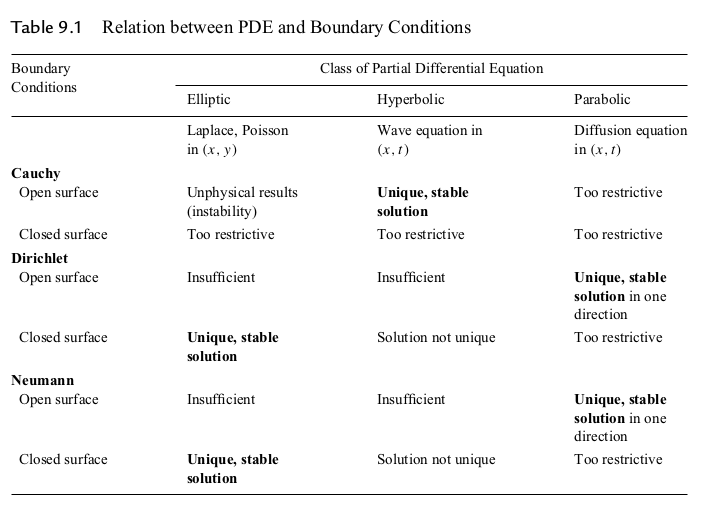
\includegraphics[width=10cm, height=7cm]{./Images/boundary.png}

\section{Integral Transforms}
Due to integration by parts, we can change derivatives to algebraic equations by integral transforms. Additionally, we have shifting property to receive answers modulo exponential.

\subsection{Fourier Transform}

\subsection{Laplace Transform}

\subsection{Legendre Transformation}
A function $f(x,y)$ can be seen as a function $g$ of $u$ and $y$ by certain transformation. (Note : $u=\frac{\partial f}{\partial x}$)

$$g = f - ux$$

\noindent This is key to going from lagrangian formalism to hamiltonian.

\section{Dirac Delta}
Any sequence of function, whose integral over all space is unity and it vanishes for all points except at zero as $n$ goes to $\infty$ will converge to dirac delta function. Extremely useful in quantum field theory.

\begin{enumerate}
  \item $\delta(x) = \frac{1}{2\pi}\int_{-\infty}^{\infty} e^{ikx} dk $
\end{enumerate}

\section{Green's Functions}

Linear differential equations have the property of superposition. Let's solve for a $\delta$ function source. If we call the solution $G$, the problem with arbitary source can be reduced to quadrature (to solving integrals), if we know $G$.

\begin{align}
  &\hat{L}(x)G(x,x') = \delta(x-x')\\
  &\hat{L}(x)u(x) = f(x)\\\nonumber
  &u(x) = \int{f(x')G(x,x')}dx'
\end{align}

Here, $hat{L}$ is a linear operator.

\chapter{Algebra}

\begin{itemize}
  \item It is useful to think of two different vector spaces, one consisting of matrices and the other of operators. One consisting of row/column vectors and the other consisting of abstract vectors. The matrices and row/column are then just representation of these abstract stuff.
  
  \item Same operator is represented by different matrices in different basis. All this matrices are connected by Similarity transformation ($S^{-1}A\,S$). Since the properties of the operator are not dependent on the basis chosen, all these matrices will share these properties. Note again that these matrices are different stuff in the vector space consisting of matrices, but they are same in a sense since they describe the same abstract operator. Therefore, they have same determinant, trace and eigenvalues (as can be easily checked). They form an equivalence class in the vector space of matrices.

  \item Inner product is an additional structure over vector space which has $3$ defining properties. 

    \begin{enumerate}
      \item Conjugate Symmerty : $<x,y> = \bar{<y,x>}$
      \item Linearity in first argument : $<ax+by,z> = a<x,z>+b<y,z>$
      \item $<x,x> > 0$
    \end{enumerate}

  \item An algbera is a vector space with product between the vectors. It is defined by $3$ additional properties
    \begin{enumerate}
      \item Right distributivity : $(x+y)z = xz + yz$
      \item Left distributivity : $z(x+y) = zx + zy$
      \item Scalar compatibility : $(ax)(by) = (ab)(xy)$
    \end{enumerate}

  \item Eigenvalues of Hermitian operator are real and eigenvectors with different eigenvalues are orthogonal. Eigenvectors are complete. (Similarly for symmetric operator).

  \item Eigenvalue of $MM\dagger$ is  \textbf{positive}. Prove by inserting the identity operator!

  \item Hermitian operators can always be diagonalized by a unitary matrix.

  \item In differential geometry, we have vector space at each point (made up by differentials).
\end{itemize}

\chapter{Asymptotics and Perturbation Methods}

$\lim_{x\to x_0} \frac{f(x)}{g(x)} = 1 := f(x) \sim g(x) \quad\mathrm{as}\quad  x\to x_0$\\

\noindent$\lim_{x\to x_0} \frac{f(x)}{g(x)} = 0 := f(x) << g(x)\quad\mathrm{as}\quad  x\to x_0$\\


\noindent Given an asymptotic sequence(each successive term having lower order) $\{\phi_i\}$ The coefficients of the assymptotic expansion 

$$ f(x) \sim a_1\phi_1(x) + a_2\phi_2(x) + ... $$

\noindent are uniquely determined.\\

\noindent If the remainder term is of lower order than the last term of the expansion for all $n$, the exapnsion is called asymptotic.\\

\noindent $\bold{Caution 1:}$ Two given functions differing by transcendentally small terms (exponentials as compared to powers) can have same asymptotic expansions. Hence, these terms are ignored in asymptotic expnsions (in powers of $x$). TST are related to essential singularities.\\

\noindent $\bold {Caution 2:}$ Need to keep higher order terms in exponentials (including sin,cos,sinh,cosh etc). Not doing so, can give wrong prefactor.\\

\noindent $\bold{Caution 3:}$ Differentiating can cause trouble too. Look at ``Tauberian Theorems" (BO - p.127)

\section{For Integrals}

\subsection{Integration by Parts}

\noindent In general, if we have

$$I(x) = \int_{a}^{b} f(t) e^{x\phi(t)} dt \quad\mathrm{as}\quad x\to\infty$$ 

$$I(x) = \int_{a}^{b} \frac{f(t)}{x\phi'(t)} d(e^{x\phi(t)})$$

$$I(x) = \frac{1}{x} \left[\frac{f(t)}{\phi(t)} e^{x\phi'(t)}\right]_{t=a}^{t=b} - \frac{1}{x}\int_{a}^{b}\frac {d}{dt}\left[\frac{f}{\phi'}\right]e^{x\phi(t)}dt $$

We hope that the second integral has lower order than the first term and that $\phi'(t)$ is not zero anywhere in the interval. This will fail when asymptotic expansion involves $log$ or fractional powers of $x$.

\subsection{Laplace's Method}

For ``sharply-peaked" integrands, where the dominant contribution comes from the nbd of a single point, we can expand the function involved in exponent around that point.\\

\noindent $\bold{Example 1 :}$

$$ I(x) = \int_{-10}^{10}e^{-xt^2}dt \quad\mathrm{as}\quad x\to\infty$$

\noindent Integration by parts won't work because $\phi'(0) = 0$. Dominant contribution comes for $t=0$. 

$$I(x) = \int_{-\infty}^{\infty}e^{-xt^2}dt - 2\int_{10}^{\infty}e^{-xt^2}dt$$

\noindent First part is simple gaussian integral, we can estimate the second integral by replacing $t^2$ bt $10t$. Which will show that the second term is transcendentally smaller than the first term.

$$I(x) \sim \sqrt{\frac{\pi}{x}}$$

\subsubsection{Stirling's Approximation :}

$$\Gamma(x+1) = \int_{0}^{\infty}t^x e^{-t}dt$$

\noindent Where's the peak of this integrand ? 

$$ \Gamma(x+1) = \int_{0}^{\infty}e^{x\log(t)-t}dt$$

\noindent Maximum occurs when the exponent is maximized, which gives $x = t$. Maximum moves with $x$. We change coordinates where it doesn't change. Define $ s = \frac{t}{x}$

$$\Gamma(x+1) = x^{x+1}\int_{0}^{\infty}e^{x\log(s) - s}ds$$

\noindent Expanding $\log$ about $s=1$.

$$\Gamma(x+1) \sim x^{x+1}\int_{0}^{\infty}e^{-x\left(1+\frac{(1-s)^2}{2}\right)}ds$$

$$\Gamma(x+1) \sim x^{x+1}e^{-x}\int_{0}^{\infty}e^{-x\frac{(1-s)^2}{2}}ds$$

\noindent We can't do this integral. But if we add TST, we have usual gaussian integral!

$$\Gamma(x+1) \sim x^{x+1}e^{-x} \sqrt{\frac{2\pi}{x}}$$

\subsection{Stationary Phase}

For an integral of the function $f(t)$ multiplied with an oscillating function, we get cancellations. If the frequency of oscillation is sufficiently big, we expect the integral to vanish. Rigorously speaking :

$$I(x) = \int_{a}^{b}f(t)e^{ix\psi(t)}dt$$

\noindent As $x\to\infty$, we try integration by parts to get


$$I(x) = \left[\frac{f(t)e^{ix\psi(t)}}{ix\psi'(t)}\right]_{t=a}^{t=b} - \frac{1}{ix}\int_{a}^{b}\frac{d}{dt}\left[\frac{f}{\psi'}\right]e^{ix\psi(t)}$$

\noindent Again, just hoping for usual conditions on $\psi'(t)$ and the second integral being of lower order, we see that 

$$I(x) \sim O\left(\frac{1}{x}\right)$$

\noindent At points when $\psi'(t) = 0$, the first order oscillation of $\psi$ vanishes, meaning it oscillates much more slowely (in second order of $t$) near this point. It gives a contribution of higher order than $O(\frac{1}{x})$. Therefore, we only integrate near neighbourhood of that point of stationary phase. After expanding around that point, a standard trick would be then to extend this region to infinity, if corresponding integral is easy to do. Since this extension would contribute to higher order terms only.

\noindent Expanding around the stationary phase ($\psi'(c) =0 $), and using Fresnel's integral(really just use Gamma function formula), we can show that if 

$$\mathrm{if}\quad f^{(i)}(c) = 0 \quad\forall i<n \quad \mathrm{then} \quad  I(x) \sim O\left(\frac{1}{x^{\frac{1}{n}}}\right)$$

\noindent A useful way to think about both the laplace and stationary phase method in a coherent manner is to see that the function multiplying $f(t)$ has an exponential order. Meaning they change much faster than $f(t)$ as long as $f(t)$ doesn't have exponential order. Note that complex representation of sin and cosine make this evident for this oscillatory functions as well. In some sense then, the integral is wholly dominated by this exponential ordered terms (including sine,cosine). Therefore we only care about the regions where this exponential ordered terms are slowly varying (given that they decay eventually in case of laplace method). In laplace method, it was the peak. In stationary phase method, it is the stationary phase.\\

\subsubsection{Bessel function}

$$J_0(x) = \frac{1}{\pi}\int_{0}^{\infty}\cos(x\sin(t)) dt$$

\noindent $\psi'(t) = 0$ at $t=\frac{\pi}{2}$. Expanding $\sin(t)$ about $t=\frac{pi}{2}$

$$\sin\left(t\right) = \sin\left(\frac{\pi}{2}\right) + \cos\left(\frac{\pi}{2}\right)\left(t-\frac{\pi}{2}\right) -\frac{1}{2}\sin\left(\frac{\pi}{2}\right)\left(t-\frac{\pi}{2}\right)^2 + ...$$

$$\mathrm{As}\quad x\to\infty$$ 
$$\frac{1}{\pi}\int_{0}^{\pi}e^{ix\sin(t)}dt\sim \frac{1}{\pi}\int_{\frac{\pi}{2}-\epsilon}^{\frac{\pi}{2}+\epsilon}e^{ix\left[1-\frac{1}{2}\left(t-\frac{\pi}{2}\right)^2 +...\right]}dt$$

\noindent As done again and again, expanding the limits of integration because it only affects higher order terms, we get 

$$J_0\left(x\right) \sim \sqrt{\frac{2}{\pi x}} \cos\left(x-\frac{\pi}{4}\right) \quad\mathrm{as}\quad x\to\infty$$

\subsubsection{Group velocity}

In quantum mechanics, we consider a superposition of waves.

$$\Psi(x,t) = \int{\phi(k)e^{i(kx-\omega(k)t)}}dk$$

\noindent What part gives the dominant contribution to the integral? The part where the phase is stationary. Giving us

$$x = \frac{d\omega}{dk} t$$

\noindent Hence, The part which gives dominant contribution to the overall integral moves with the velocity $\frac{d\omega}{dk}$.

\subsection{Steepest Descent}
This method makes previous two methods a consequence. Consider the integral 

$$I(x) = \int_{C}h(t)\, e^{x\phi(t)}\, e^{ix\psi(t)}$$

\noindent If we choose a contour such that the $\psi(t)$ is constant on this contour, we can bring it out of the integral and use laplace's method. This will enable us to find higher order terms that we missed in stationary phase method. Please check the video by Professor Strogatz for example.\\

\chapter{Groups}

\section{Finite Groups}

\noindent\textbf{Once and Only Once Rule:} In the multiplication table, each row or each column contains each element of the group exactly once. Try constructing all posible finite groups of order n.\\

\noindent\textbf{Lagrange's Theorem:} Order of every subgroup divides the order of original group. (Using disjointness of cosets)\\

\noindent\textbf{Centre:} The set defined by elements $z_i$ such that $z_i$ commutes with all elements of the group is an abelian subgroup of $G$.\\

\noindent\textbf{Permutations:} A permutation can be decomposed into product of two cycles. It's even or odd depending on number of two cycles present. (Imagine the ball hiding guy arranging the glasses. He achieves all sort of permutation by doing exchanges again and again). Odd and even because matrix representation corresponds to elementary operations which have determinants $1$ or $-1$.\\

\noindent\textbf{Cayley's Theorem:} Any finite group $G$ with $n$ elements is isomorphic to a subgroup of $S_n$ (Permutation Group). (Associate each $g_i$ with corresponding permutation by checking the permutation offered by observing the multiplication table.)\\

\noindent\textbf{Conjugation:} Two elements $g$ and $g'$ are similar if there exists an element $f$ such that $f^{-1}gf = g'$. Conjugation is an equivalence relation, therefore we can form equivalence classes. (Doing something, doing main thing, undoing something leads to a similar element in some sense. Which is what defines this relation). Equivalence classes provide disjoint partitions of the set (Simple proof). Equivalence relations provide a zoom out lens of a given set.\\

\noindent\textbf{Invariant Subgroup:} Say $H$ is a group. Conjugate $H$ with some $g$ not in $H$. It will give another group. Conjugation will lend to similar elements but not same. If the conjugated group is same as the original group \textbf{for all g}. Then that group is special, and rightly deserves the name Invariant subgroup. All elements equivalent to elements in the subgroup $H$ are also in $H$. It's a sort of an equivalence relation that preserves the group structure.\\

\noindent\textbf{Quotient Group:} If $G$ has an invariant subgroup $H$, we can form another group consisting of left cosets $g_aH$ as elements called the Quotient group $G/H$. We can zoom out sets using equivalence relation, in the same way we need invariant subgroups to zoom out of the group if we want to preserve the group strucutre. It's a somewhat stronger condition than just using equivalence class to zoom out in order to keep group structure. \\

\noindent\textbf{Automorphism Group} An isomorphism between $G$ to $G$ is called an automorphism. Different automorphisms form a group under composition of automorphisms. It is denoted by $Aut(G)$ We can check that $\phi_a$ defined by conjugation with $a$ ($\phi_a(g) = aga^{-1}$) is an automorphism. Automorphisms of this type are called inner automorphisms. \textbf{Inner automorphisms form a normal subgroup of $Aut(G)$}.

\section{Rotations and Lie Algebra}

Calculus is mankind's greatest invention. We analyze behaviours of functions in infinitesimal neighbourhood and then form differential equations to find the right relationship (from infinitesimals to reals). Taylor series is, in a sense $f(x+\Delta x) = exp(\Delta x\frac{d}{dx})f(x)$. For groups, the higher derivatives $\frac{d^n}{dx^n}$ are simple matrix multiplication of the generator $\frac{d}{dx}$. Rotation is defined by

$$R^{T}R = I \quad det(R) = 1$$

\noindent Check that generators are antisymmetric matrices. We stick in $-i$ to make the generators hermitian.

\subsection{Lie Algebra}

Instead of looking at the actual elements of the group, we are now concerned with generators only. We can go back to the actual group using exponention. For instance, $SO(n)$ generators are antisymmetric matrices. A general antisymmetric matrix can be seen as linear combination of $\frac{n(n-1)}{2}$ antisymmetric matrices. Now you know why lorentz group is $6$ parameters group. It is a weird kind of rotation in $4$ dimenstion.\\

\noindent The structure of the group is determined by the commutation relation of the generator. Commutation relation of the generators form an algebra which is called lie algebra of the cooresponding lie group.

$$[J_i, J_j] = i\epsilon\indices{_i_j_k}J_k$$

\noindent We can do something like this for all sorts of lie groups. Where $\epsilon$ are replaced by some other constants known as the structure cosntatnts.\\

\noindent To see how, consider the product of two group elements near identity $A(\alpha)A(\beta)$, the product itself is a group element with different parameter $\gamma$. Compare $A(\gamma)$ with with the result of previous product, which will give you a closed relation between the commutators. When you read theory of lie, you will understand that infinitesimal generator corresponding to each parameter is a vector. We have now identified a way to multiply these vectors (with three specific rules required for a vector space to be an algebra). The structure constants will be different for different choice of basis.

\section{Representation Theory}

It's useful to represent the group elements $g$ as matrices which preserve the multiplication structure of the group. Namely,

$$D(g_1 g_2) = D(g_1)D(g_2)$$

\noindent Obviously, $D(g) = 1$ (one dimensional identity matrix) is a perfectly good representation. There's a loss of information in some sense. $D$ is homomorphism as is written, but if it is an isomorphism, we say that the representation is faithful (useful). Since every finite group is a subgroup of $S_n$, and $S_n$ has obvious representation of dimension $n$, we have faithful representations of every finite group. (A bit complicated for continuous groups, but we're physicists)

\subsection{Character is a function of class}

$$\chi^{(r)}(g) = Tr(D^{(r)}(g))$$

\noindent There may be many representations of the same group. We denote a particular representation $r$ by $D^{(r)}$. Character of a particular element under a given representation is the trace of $D^{(r)}(g)$ , and is denoted by $\chi^{(r)}(g)$. It's easy to prove that \textbf{character of an entire equivalence class is same.} (Using cyclic property of trace).

\subsection{Equivalent represntation} 

There may be more than one representation of a given group. Clearly, We are only concerned with reducible representations. Even among the reducible representations, given a representation $D(g)$, we can construct another representation $D'(g) = S^{-1} D(g) S$ (check that $D'$ is really a presentation). These representations are esentially the same connected by similarity transformation. If we are given two represenations, are they same? One thing you can check is that the character is invariant under the representations connected by similarity transformation. Therefore, if each matrix was conjugated (similarly transformed) and we were to be presented with weird looking set of matrices as representation, they may just be realted to some simple looking set of matrices via similarity transformation.

\subsection{Irreducible or Reducible}

The dimension of the matrix is said to be the dimension of repersentation. You can make any dimensional representation just by direct summing $1$ dimensional trivial representation. (Note that the direct sum of two operators acts independently on the vectors from the direct summed vector spaces, in matrix language, it will be a block diagonal matrix and the vector will be an extended row). Although, by similarity transformation in higher dimension, we could make this block diagonal matrices uglier, and it will be messy to see if the representation is irreducible. In any case, ideally we say that the representation is irreducible no subspace of that representation is also a representation. Goal is to figure out the number of irreducible representations.

\chapter{Theory of Lie}

All functions considered are smooth etc. $x$ without subscript inside the function is to be seen as something which involves all $x_i$. Imagine a flat space and cartesian coordinates of dimension $n$. Now consider, a set of transformations (Called point transformation)

$$x'_i = f_i(x_1, x_2, x_3, ...) \quad \forall i \in {1,2,..n}$$

\noindent We can imagine $x$ moving to $x'$ in the same system or a region in the domain of $x$ system being mapped to a correesponding region of $x'$ system.\\

\noindent We wish to see this transformation as a continous group. What do we need? We want it to be invertible. Which demands usual condition of Jacobian being non-zero under the region of consideration (Chapter 1 final theorem). Further, if we were to transform twice using different parameters, we should end up in the same family. Let's introduce a notation for finite parameter continuous group to make this more clear. \\

\noindent A continuous transformation involving finite parameters will be represented as $x' = f(x;a)$. For this family to form a group, we demand that $x'' = f(x'; b) = f(x;c)$. Now if we have a $r$ parameter transformation 

$$x'_i = f_i(x_1,x_2,...; a_1,a_2,...,a_r)$$

\noindent We can eliminate the constants to form a set of differential equations for $x'_i$. This differential equations will have an amazing property. Namely, if we find two different set of families of solution $x'_i = g_i(x;b_1,b_2,...,b_r)$ and $x'_i = h_i(x;a)$. Then the composition $y'_i = g_i(h_1(x,a), h_2(x,a),...;b_1,b_2,...,b_r)$ is also a solution by definition of the group property of initial equation.\\

\noindent A function $f$ in $x$ system may look very different in $x'$ system. If it looks the same, we say that the trasformation which takes $x$ to $x'$ is a symmetry of $f$. The magic in theory of continuous groups is that we can always analyze upto the first order near identity, namely, we are dealing with generators only. An explicit example is considered below (Section of Killing Vectors).\\

\noindent More generally, let $x$ be transformed to $y$ and $u_i(x)$ be transformed to different functions under the group action, which in $y$ coordinates, have the form $v(y)$, then the function $P(x,\frac{\partial u}{\partial x}, \frac{\partial ^2 u}{\partial x^2},...)$ is an invariant of the group if 

$$ P\left(x,\frac{\partial u}{\partial x}, \frac{\partial ^2 u}{\partial x^2},...\right) = P\left(y,\frac{\partial v}{\partial y}, \frac{\partial ^2 v}{\partial y^2},...\right)$$

\section{Infinitesimal Transformation and Vector field generating the Transformation}

Consider the $n$ parameter transformation, let's think of infinitesimal increment $\epsilon$ of the parameterk $k$, all the rest of parameters are chosen such that it corresponds to identity transformation.

\begin{align}
x'_i = f_i(x;e_1,...,e_k+\epsilon,...,e_n)
= x_i + \frac{\partial f_i}{\partial a_k} (x;e)\epsilon + ... \quad(i = 1...n)
\end{align}

\noindent If we introduce the vector field

$$X\indices{^e_k} = \sum_{i=1}^{n} \frac{\partial f_i}{\partial a_k}(x;e) \frac{\partial}{\partial x_i} := \sum_{i=1}^{n}\xi_{ki}(x)\frac{\partial}{\partial x_i}$$

\noindent We have $x'_i = x_i + \epsilon \xi_{ki} + ... \quad (i=1...n)$\\

\noindent More generally, arbitary increments from identity to all parameters $(e_1 + \epsilon\lambda_1,...,e_k+\epsilon\lambda_k,...e_r+\epsilon\lambda_r)$ will give

\begin{gather}
x' = x + \epsilon X +...\\
X := \lambda_1 X_1^e + \lambda_1 X_2^e+...
\end{gather}

Clearly, the infinitesimal generators are vectors at each point of the manifold (Since $dx$ is a vector always). 

\section{A brief note on invariance}

There's a deep but trivial connection between the coordinate transformation that preserve the form of the function and the symmetry of the function. As stressed many times, Transformation we will consider are infinitesimal (Finite can be generated easily from them).\\

\noindent Say we have a new coordinate system $x' = x + \epsilon \, \eta(x)$. Any function $f(x)$ will have a totally different form $f'(x')$. Here, $x$ and $x'$ refer to the same point on the manifold, but in different coordinate systems. Hence, the numerical value of two expression is same $f'(x') = f(x)$. However, if we want the form of the function itself to be the same in new coordinate system, we need $f'(x') = f(x')$. But if the transformation $x'=x'(x)$ is such that $f(x') = f(x)$ then we clearly have $f'(x') = f(x')$. Such transformation for which $f(x') = f(x)$ are called infinitesimal symmetry of the function. Therefore, the infinitesimal transformations which doesn't change the value of the function are the corresponding coordinate transformations which preserve the form of the function under coordinate transformations. It's trivial, but took me long to realise.\\

\noindent In Noether's theorem, think of coordinate tranformations as active transformations (meaning that we bring the field backwards, instead of moving the coordinates forward. So both, coordinate and field transformations correspond to the field transformation effectively. The reason I want you to think in terms of active transformation is because I don't want you to get confused with the definition of Scalars (Especially the notation). In our notation, $f'(x') = f(x)$ is always true where $'$ denotes $f$ in new coordinates. Notation $'$ is  used to describe the new (varied) field in many books. Varied field is a different scalar field altogether, in this notation $'$ is not describing the same field in new coordinates but the different field in same coordinates.

\subsection{Killing vectors}

Consider finding out symmetries of the metric in relativity. We consider an infinitesimal transformation at all coordinates

$${x'}\indices{^\mu} = x\indices{^\mu} + \epsilon \, \eta\indices{^\mu}(x)$$

\noindent Here, $\eta\indices{^\mu}(x)$ is like $dx\indices{^\mu}$, hence it can be treated as vector. Namely, its indices can be lowered and uppered. Note also, that the inverse transformation can be given by (since first order change inside the function $\eta$ will give second order overall change)


$$x\indices{^\mu} = {x'}\indices{^\mu} - \epsilon \, \eta\indices{^\mu}(x')$$

\noindent The metric transforms under general coordinate transformation as 

$${g'}\indices{_\alpha_ \beta}(x') = g\indices{_\mu _\nu}(x)\frac{\partial x\indices{^\mu}}{\partial {x'}\indices{^\alpha}} \frac{\partial x\indices{^\nu}}{\partial {x'}\indices{^\beta}}$$

\noindent We want the metric to keep the same form under such coordinate transformation, meaning that we want ${g'}\indices{_\alpha_ \beta}(x') = g\indices{_\alpha_ \beta}(x')$. This connects the $x$ system and $x'$ system in a sense. Equation says that the point $x$(system 1) in the manifold which is also the point $x'$(system 2) in different system is related to the point $x'$(system 1) of the original system in this fashion. 

$$g\indices{_\alpha_ \beta}(x) + \epsilon \, \partial_\sigma g\indices{_\alpha_ \beta} \, \eta\indices{^\sigma}(x)= g\indices{_\mu_ \nu}(x) \left[\delta\indices{^\mu_\alpha} -\epsilon \, \partial_\alpha\eta\indices{^\mu}\right] \left[\delta\indices{^\nu_ \beta} -\epsilon \, \partial_ \beta\eta\indices{^\nu}\right]  $$

\noindent Here, we have ignored $\epsilon^2$ terms arising from partial derivatives of $\eta$ evaluated at infinitesimally different point. Which will give us a coordinate independent equation for vector $\eta\indices{^\mu}$

\begin{equation}
\nabla\indices{_\mu}\eta\indices{_\nu} + \nabla\indices{_\nu}\eta\indices{_\mu} = 0 
\end{equation}

\noindent The vector field $\eta$ is then the generator of the continuous symmetry of the metric.

\section{Lie Algebra}

It can be shown that the infinitesimal generators form the relation

$$[X_ \rho, X_\sigma] = c\indices{^{\tau}_ \rho_\sigma}X_\tau$$

\noindent With $c\indices{^\tau_ \rho_\sigma} = -c\indices{^\tau_ \sigma_ \rho}$. Further, they satisfy the Jacobi identity

$$[X_ \rho,[X_\sigma,X_\nu]]+ [X_ \sigma,[X_\nu,X_ \rho]] + [X_ \nu,[X_ \rho,X_\sigma]] = 0 $$

\noindent Such a vector space with product defined as above form Lie algebra (Tangent space at the identity element of the manifold). Note that we can also realize matrices to represent the same thing, but the generators are vectors in reality. Matrices are just represerntations. Formally, the lie algebra has following three prperties

\begin{gather}
  [\alpha X + \beta Y, Z] = \alpha[X,Z]+\beta[Y,Z]\\
  [X,Y]+[Y,X] = 0\\
  [X,[Y,Z]]+[Y,[Z,X]]+[Z,[X,Y]] = 0
\end{gather}

\noindent Under a transformation of basis (using matrix $a\indices{^\nu_ \rho}$), the structure constants change as 

$${c'}\indices{^\tau _ \rho_\sigma} = a\indices{^\nu_ \rho}a\indices{^\lambda_ \sigma}c\indices{^\kappa _\nu_\lambda} (a\indices{^\kappa _\tau})^{-1}$$

\noindent \textbf{Different Lie groups may have the same structure constants and as a result the same Lie algebra, but be radically different groups globally}. Groups possessing common lie algebra are said to be locally isomorpihc, that is, isomorphic in the neighbourhood of the identity. The Lie algebra $su(2)$ and $so(3)$ are isomorphic while the Lie groups $SU(2)$ and $SO(3)$ are only locally isomorphic. A radical example is $SO(2)$ and $T(1)$ have single selfcommuting generator but the groups are obviously not isomorphic globally.

\subsection{Subalgebras, Ideals and Proper Ideals}

If a subspace $Z$ (as a vector subspace) of lie algebra $A$ is closed, it's a subalgebra.

$$[X,Y]\in Z \quad \textrm{for\, any} \quad (X,Y \in Z)$$

\noindent A subset $Z$ is ideal (or invariant subalgebra) of $A$ if it is closed under product with another element in $A$. This is analogous to the invariant subgroup which remains as it is under conjugation by any element.

$$[X,Y]\in Z \quad \textrm{for\, any} \quad (X\in Z, Y \in A)$$

\noindent that is,

$$[X_ \rho, X_ \sigma] = c\indices{^\tau_ \rho_\sigma}X_\tau \quad (\rho,\tau \in Z, \sigma\in A)$$

\noindent If the algeba has members which are not in the ideal, the ideal is called proper ideal. Basically, it is not the whole agebra itself.\\

\noindent We had a concept of abelian group. In close analogy, a subalgebra $Z$ is abelian if commutator $[X,Y]=0$ for any $(X,Y \in Z)$. Similarly, we had a concept of center (the set of elements which commute with all other elemnts of the group). In close analogy, the set of all elements $X_\sigma$ of algebra $A$ is said to form the maximal ideal or center of the algebra if $[X_ \rho, X_\sigma] = 0 \quad (\rho\in Z, \sigma\in A)$.\\

\noindent Basically, we tried to see the product of vectors as some group theoretic multiplication and tried to identify corresponding things here.



\chapter{Classical Mechanics}

\section{Lagrange Multipliers}

How would you find the max/min of a function $f(x,y)$? We get two equations by setting both partial derivatives equal to zero. We can simply solve for $x$ and $y$. Now if there's a constraint of the form $g(x,y)=c$, it may happen that the solution $(x_0,y_0)$ doesn't lie on $g$. What can we do? We introduce additional parameter $\lambda$ to adjust itself so as to make $x$ and $y$ fit on $g$. We find max/min for $f'(x,y)=f(x,y)+\lambda g(x,y)$, this maximum will depend on the parameter $\lambda$. We can then impose $g(x,y)=c$ to solve for $x,y,\lambda$. \\

\noindent Geometric intuition for lagrange multipliers is that the change in $f$ is maximum along the gradient of $f$. If, along the curve $g$, there's a point where gradient of $f$ is parallel to gradient of $g$, then moving along $g$ will give min/max change in $f$ at that point (it's like $f$ has min/max at that point as seen by $g$, the contour lines just touch).\\

\noindent Consider the action 

$$S = \int L(q,\dot{q},t) dt$$

\noindent If we have $n$ constraint realtion of the form $\sum_{k}a_{ik} dq_k = 0$, we can introduce $n$ additional parameters $\lambda_i$ and add all these terms in the variation of orginal $\delta L$.

\section{General remarks}

\begin{itemize}
  \item If $q_k$ does not appear in the lagrangian, we have conserved quantity(constant of motion) corresponding to it. However, We cannot directly substitute this conserved quantity back into the lagrangian and then use euler lagrange equations for other coordinates. Because, (firstly, the form of new lagrangian is clearly different from original, so there's no reason to believe it would work anyway) the euler-lagrange equations were derived based on the assumption that the coordinates $q_i$'s are independent(David Tong Ch2, p.29). In that sense, even though $q_k$ is a ignorable in lagrangian formalism, it cannot really be ignored when we wish to derive equations of motion. In Hamiltonian formalism, if $q_k$ is ignorable, then it is truly ignorable in the sense that $p_k$ can be substituted for a constant in the hamiltonian, and problem becomes $n-1$ dimensional one.

\begin{align}
&L = L(q_1,q_2,...q_{n-1};\dot{q1},...,\dot{q_n};t)\\
&H = H(q_1,q_2,...q_{n-1}; p_1,...,p_{n-1};\alpha;t)
\end{align}

The motion of $n$th coordinate can simply be given by 

$$\dot{q_n} = \frac{\partial H}{\partial\alpha}$$

  \item A beautiful geometric interpretation of noether theorem can be found on Wikipedia. In summary, if the action doesn't change under some transformation, since first order changes around equation of motion doesn't change action, a 'slanting term' would be conserved.
\end{itemize}

\section{Small Oscillations and Stability}

Consider $\ddot{x} = f(x)$. Point $x_0$ is called stable if $f(x_0) = 0$. For if initial conditions were $x=x_0$ and $\dot{x} = 0$, the system would stay at $x_0$. Consider small oscillations $x = x_0 + \eta(t)$ about this point. Upto the first order, 

$$\ddot{\eta} = f'(x_0)\eta$$

\noindent In case $f'(x_0) < 0$, the solution is oscillatory, otherwise exponential. It's just about linear second order system now. Let's see this in more dimensions

$$\ddot{q_i} = f_i(q_1,q_2,...)$$

\noindent Equilibrium point $q_i^{0}$ satisfies $f_i(q_1^0,...,q_n^0)$ for all $i=1...n$. Expanding about this point, we get again

$$\boldsymbol{\ddot{\eta}} = F \boldsymbol{\eta}$$

\noindent Here $F$ is seen to be a matrix $\frac{\partial f_i}{\partial q_j}$ evaluated at the equilibrium point. In one dimension we only cared about the sign of this matrix to check for stability. In higher dimension, the analysis depends on the nature of this matrix. If we assume that the matrix is symmetric, then it has complete set of orthogonal eigenvectors with real eigenvalues. If $\boldsymbol{\mu_a}$ are the eignevectors of $F$ with eigenvalue $\lambda_a^2$, that is $F\boldsymbol{\mu_a}= \lambda_a^2\boldsymbol{\mu_a}$. As you may have guessed, the solution depends on the eigenvectors like

$$\eta(t) = \sum_{a}\boldsymbol{\mu_a}\left[A_ae^{\lambda_a t} + B_ae^{-\lambda_a t}\right]$$

\noindent The system will be stable only if all eigenvalues are negative. Further, the special vectors $\boldsymbol{\mu_a}$ that have arisen out of beautiful combination of linear algebra and differential equation are called normal modes of the system. The most general solution has the form

$$\boldsymbol{\eta} = \sum_{a,\lambda_a^2>0}\boldsymbol{\mu_a}\left[ A_ae^{\lambda_a t} + B_ae^{-\lambda_a t}\right] + \sum_{a,\lambda_a^2<0}\boldsymbol{\mu_a}A_a cos(\omega_a(t-t_a))$$

\section{A comparision of Hamiltonian and Lagrangian Formalism}

We have $n$ second order equations in lagrangian formalism. Unfortunately, the lagrangian is considered to be a function of $2n$ coordinates, where last $n$ coordinates are NOT REALLY on an independent footing from first $n$ coordinates. By legendre transformation, we arrive at a formalism where we can have $2n$ truly independent coordinates and the equation of motion becomes $2n$ coupled first order. It can be shown that euler-lagrange equation do not change their form under point transformation. The analogy of point transformations in hamiltonian formalism are cannonical transformations. In hamiltonian formalism, we have $2n$ independent coordinates which can all be pointwise transformed, unlinke only $n$ coordinates in the lagrangian formalism. However, not all such transformation preserve the form of the equation. Those which do, are called cannonical transformations.

\subsection{Cannonical Transformation}

In phase space, we can associate a $2n$ dimensional vector $\boldsymbol{x}$ corresponding to the coordinates $(q_1,...,q_n,p_1,...,p_n)$. The hamilton's equation are then simply

$$\boldsymbol{\dot{x}} = J\frac{\partial H}{\partial \boldsymbol{x}}$$

\noindent where $ J = \begin{pmatrix}
  0 & 1\\
  -1 & 0
\end{pmatrix}$

\noindent Let's make a point transformation $x \rightarrow y(x)$ in phase space and check if the equation of motion have the same form.

$$\boldsymbol{\dot{y}} = \mathbb{J}J\mathbb{J}^T\frac{\partial H}{\partial \boldsymbol{y}}$$

\noindent Here $\mathbb{J}_{ij} = \frac{\partial y^i}{\partial x^j}$. To have the same form in $y$

$$\mathbb{J}J\mathbb{J}^T = J$$

\noindent Transformations whose jacobian have these form are called canonical. Rings bell from group theory? Already thinking about generators and infinitesimal transformations? Further, we can show that poisson brackets remain invariant under cannonical transformation in a sense that you can calculate them in any particular coordinate system (connected by cannonical transformation) you like. Don't they give you a feeling of dot product (quadratic form so to speak)? It's kind of a scalar on some manifold? Like in general relativity $\partial_\mu\phi\partial^\mu\phi$ is a scalar. (Tong p.101 last chapter)\\. The associated symmetry group (for cannonical transformation) is called symplectic group. (Check Classical Groups wyborne P.14).

\noindent Converse is also true. That is, if transformations are such that they preserve the cannonical commutation relations $(\{Q_i,Q_j\}=0, \{Q_i,P_j\}=\delta_{ij})$, these transformations are cannonical.\\

\noindent Now, Lie's theory is everywhere. Until now, we thought of cannonical transformation as such coordinate transformations which preserve the form of the hamilton's equation. Just like how lorentz invariant metric preserves the form of equations. Infinitestimal cannonical transformation can also be thought of as active (acting on the same coordinate system). They take $(q_i,p_i)$ to a different point $(q_i+\epsilon E_i, p_i+\epsilon F_i)$. For this transformation to be cannonical, we can show that it has to be in the form $(q_i+\epsilon\frac{\partial G}{\partial p_i}, p_i-\epsilon\frac{\partial G}{\partial q_i})$. $G(q,p)$ is called the generating function. For example, if $G = p_k$, $q_i \rightarrow q_i+\epsilon\delta_{ik}$ and $p_i\rightarrow p_i$. We say that momentum is a generator of translation.


\chapter{Quantum Mechanics}

\begin{itemize}

  \item A state of quantum system is defined by a ket $\ket{\psi}$ or the corresponding bra $\bra{\psi}$ (For every vector space, we can construct a dual space (of linear functionals)). There is a one-one correspondence between this space.

  \noindent \textbf {Pedantry} : If $V$ is a finite dimensional vector space, its dual $V^*$ has the same dimension. Therefore, they're isomorphic. (Note that finite dimensional vector spaces with same dimensions are obviously isomorphic.) By establishing the dual basis, we establish this isomorphism between $V$ and $V^*$. But this isomorphism is not natural. However, if we have an inner product space, we can have almost natural isomorphism between a vector $\ket{\alpha}$ and its dual, $\bra{\alpha}$ is naturally defined by fixing the first element of inner product as $\ket{\alpha}$.

  \item Inner product is positive definite and has conjugate symmetry by defintion. Important for probabilistic interpreation :
    $$\bra{\alpha}\ket{\beta} = \bra{\beta}\ket{\alpha}^* \quad \textrm{and} \quad \bra{\alpha}\ket{\alpha} \ge 0$$ 

  \item The eigenvalues of a Hermitian operator are real and Eigenkets corresponding to different eigenvalues are orthogonal. Every observable corresponds to a Hermitian operator. Converse, I am not aware of yet. \\

  \textbf{Postulate:} The eigenkets of an observable are complete. This is a physical requirement, not a mathematical truth. As a consequence, we start by identifying the observables, and since they're hermitian, we choose an orthonormal basis consisting of eigenkets of this observable, which will span the entire hilbert space.

\item If $[A,B] = 0$, every eigenvector of $A$ is an eigenvector of $B$ and vice versa.

\item Given two sets of orthonormal base kets ${\ket{a^{(i)}}}$ and ${\ket{b^{(i)}}}$, there is a unitary operator

  $$U = \sum_{k} \ket{b^{(k)}}\bra{a^{(k)}}$$

  such that $\ket{b^{(i)}} = U\ket{a^{(i)}}$

  Check $U^\dag U = I$

\item Matrix representation of the same operator in different basis are connected by similarity transformations $X' =U^{-1}XU$. LHS is the matrix of operator in new basis, RHS are matrices in old basis. If both basis are orthonormal, the matrix $U$ is unitary. Trace is a property of the operator, not of the basis (Although we are only talking about transformations connecting orthonormal basis here, it's true for general transformation because of the cyclic property of trace). \textbf{Every hermitian matrix is unitary diagonalizable.}\\

\item Similarity transformation are much more general. As we know, all finite vector spaces of a given dimension are isomorphic to each other. Similarity transformation connects two matrices $A$ and $B$ by an invertible matrix $P$(change of basis matrix) such that $B = P^{-1}AP$. In general linear group $GL(n,\mathbb{C})$, this is same as conjugation that we discussed in group theory. Character is same for an entire equivalence class means that trace is same for all matrices connected by similarity transformation. In linear algebra language, they represent same operator in different basis.\\

\item There is a minor contextual linguistic difficulty here. When seen purely as a group $GL(n)$, the matrices connected by similarity transformation form an equivalence class. When this group is seen to be acting on an abstract vector space, all the elements of equivalence class represent the same operator(acting on this abstract vector space) in different basis. We can naturally ask, is there a relation between operators connected by unitary transformation (Note that it is different from the representation of same operator in different basis). There is a theorem which says that operators connected by similarity transformation are physically the same (Sakurai pp. 39).\\

\item In summary, it is useful to associate the matrix representation to elements of $GL(n)$, which I call pure matrices. Think of operators as abstract quantities then, which are represented by an entire equivalence class of $GL(n)$.


\end{itemize}

\section{Difference between direct sum(product) and tensor product}

\noindent Direct sum of two vector spaces $A$ and $B$ is such that $(a,b)\, \textrm{with} \, a\in A, b\in B$ and $(ca, b)$ is considered diferent from $(a,cb)$ (Imagine $\mathbb{R}\bigoplus\mathbb{R} = \mathbb{R}^2$, both are different vectors in $\mathbb{R}^2$). We don't need to explain anything, they act as independent vector spaces and it's simple. For Direct Product, we need to restrict the structure by defining properties for the product. The dimension of Direct Sum of vector spaces add, they multiply in case of tensor product.\\

\noindent Fundamental property defining tensor product of vectors is following (which is not true for direct sum(product))

\begin{gather}
  (\alpha v) \otimes w = \alpha (v \otimes w) = v \otimes (\alpha w)\notag \\
  (v_1+v_2)\otimes w = v_1\otimes w + v_2\otimes w 
\end{gather}

\noindent If $V$ has basis $(e_1,e_2,..)$ and $W$ has basis $(f_1,f_2,...)$ then $(e_i\otimes f_j)$ is basis for $V\bigotimes W$. Tensor produt of oprtators is defined in the natural way. \\

\noindent Inner product is also defined most naturally.

$$\braket{\sum_{ij}a_{ij}v_i\otimes w_j}{\sum_{pq}b_{pq}v_p\otimes w_q} = \sum_{ij}\sum_{pq}a^{*}_{ij}b_{pq}\braket{v_i}{v_p}_V\braket{w_j}{w_q}_W$$

\section{Quantum Teleportation}

We note that the pauli matrices are both hermitian unitary, and can be realized physically as hamiltonians by setting up appropriate magnetic field. We cannot have a unitary operator which clones the state (No cloning theorem). 


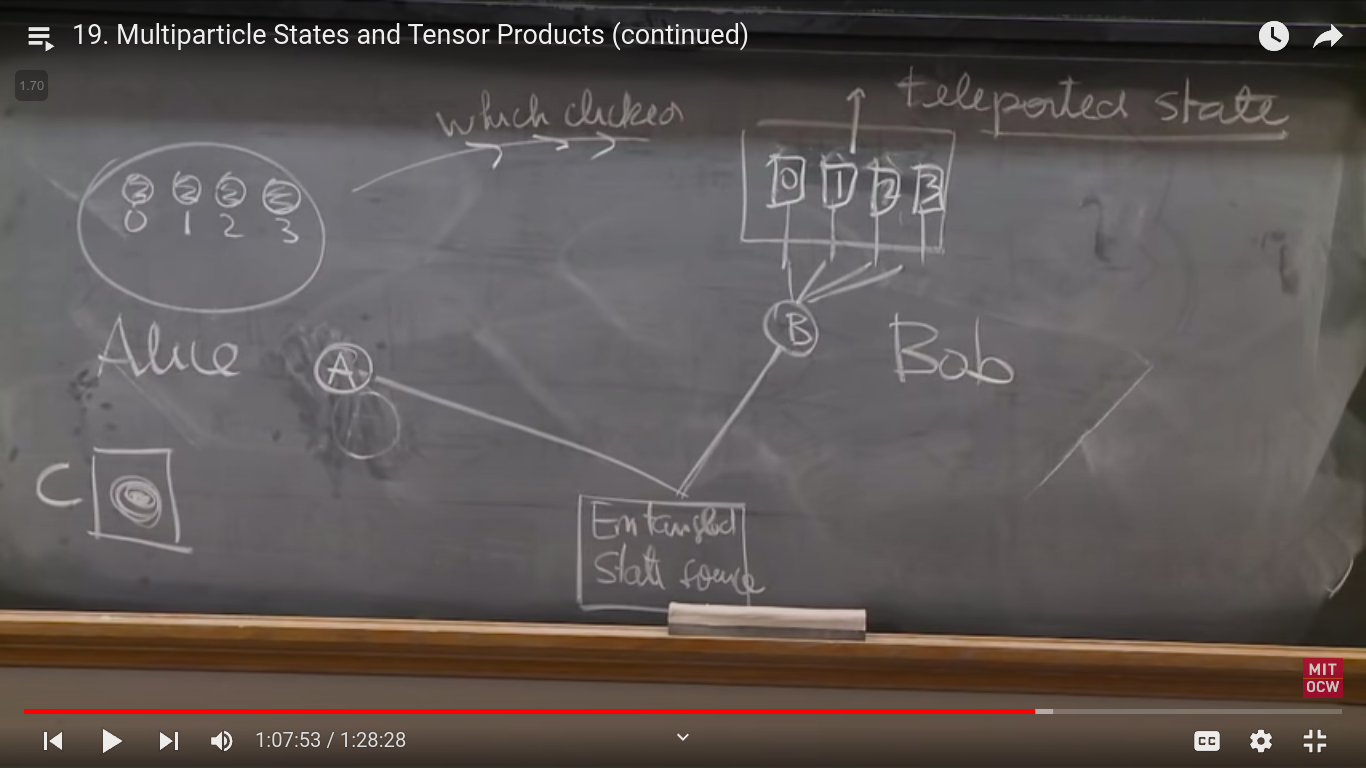
\includegraphics[width=11cm, height=7cm]{./Images/Teleportation.png}\\

\noindent Say Alice wants to teleport the state $(\alpha\ket{+}_C+\beta\ket{-}_C)$. We use an auxiliary entangled state (we use ${\ket{\Phi_i}}$ to denote the bell basis)

$$\ket{\Phi_0} = \frac{1}{\sqrt{2}}(\ket{+}_A \ket{+}_B + \ket{-}_A\ket{-}_B)$$

\noindent The total state $\ket{\Psi}_{T} = \ket{\Phi_0}_{AB}\otimes (\alpha\ket{+}_C+\beta\ket{-}_C)$ is (by trivial algebra)

\begin{align}
  \ket{\Psi_T} &= \frac{1}{2}\ket{\Phi_0}_{AC}(\alpha\ket{+}_B + \beta\ket{-}_{B})\\
                                   & + \frac{1}{2}\ket{\Phi_1}_{AC}(\beta\ket{+}_B + \alpha\ket{-}_{B})\nonumber\\
                                   & + \frac{1}{2}\ket{\Phi_2}_{AC}(i\alpha\ket{-}_B + i\beta\ket{+}_{B})\nonumber\\
                                   & + \frac{1}{2}\ket{\Phi_3}_{AC}(\alpha\ket{+}_B - \beta\ket{-}_{B})\nonumber
\end{align}

\noindent Alice measures the bell state. She sends this information to bob classically. Corresponding to each bell state that Alice measures, Bob can set up appropriate magnetic field to get the original state.

\section{Baker-Hausdorff Lemma}

In Heisenberg picture, the operators (and therefore, their eigenkets) evolve with time. The state ket remains what it was at $t=0$. In schrodinger picture, the operators are what they are, the state ket evolves according to the hamiltonian. Now, how do we evaluate the operator after finite time $t$ in Heisenberg picture?

$$A(t) = exp\left(\frac{iHt}{\hbar}\right)A(0)\,exp\left(\frac{-iHt}{\hbar}\right)$$

Prove the following :

\begin{align}
  exp(iG\lambda)\,A\,exp&(-iG\lambda) = A + i\lambda[G,A] + \left(\frac{i^2\lambda^2}{2!}\right)[G,[G,A]]\\
                    & +...+\left(\frac{i^n\lambda^n}{n!}\right)[G,[G,[G,...[G,A]]]...]+...\nonumber
\end{align}

\noindent Since we have an algbra, every commutator will be some combination of the elements of the algebra. Therefore, we only need to know commutators of the algebra for finite transformations (elements of the actual group). This is just theory of lie.

\section{Angular Momentum}

Momentum is the generator of translation in space, Hamiltonian is the generator of translation in time, Angular momentum is the generator of rotations.\\

\noindent Tranlsations in different directions commute, therefore $[p_i,p_j] = 0$ (please derive). Rotation in different directions don't commute, so we have a different algebra for their generators. This algebra defines everything.

\subsection{Operator Vector Analysis}

\noindent If $\vec{a} \, \mathrm{and} \, \vec{b}$ are vector operators,  we have

\begin{align}
&\vec{a}\cdot\vec{b} = a_ib_i \quad \mathrm{(definition)}\\
&\vec{a}\cdot\vec{b} = \vec{b}\cdot\vec{a} + [a_i,b_i]\\
&\vec{a}\times\vec{b} = -\vec{b}\times\vec{a} + \epsilon_{ijk}[a_j,b_k]
\end{align}

\noindent Of course, not any pair of operators can be considered vector. An operator $V$ is a vector operator if its expectation values transform as real vectors under rotation (Turn it into mathematical definition (Sakurai p.246)). We simply state the definition\\

$$[L_i, U_j]  = i\hbar\epsilon_{ijk}U_k$$

\noindent We can show that if $\vec{u}$ and $\vec{v}$ are vector operators under rotation, $\vec{u}\cdot\vec{v}$ is a scalar(commutator with $L_i$ is zero) and $\vec{u}\times\vec{v}$ is a vector. For practice, show that $\vec{r}\, \mathrm{and}\, \vec{p}$ are vector under rotation.

\section{Addition of Angular Momentum}

If $J^{(1)}$ is angular momentum in space $V_1$ and $J_2$ is angular momentum in space $V_2$ then $J = J^{(1)}\bigotimes\mathbb{1} + \mathbb{1}\bigotimes J^{(2)}$ is angular momentum in space $V_1\bigotimes V_2$ (Check algebra).

\subsection{Spin Orbit Coupling}

(Check out thomas precession. It's beautiful) Consider hydrogen atom. Since electron has intrinsic spin, due to the motion of proton around electron, there will be a magnetic field which changes the energy by $\Delta H = \vec{\mu}\cdot \vec{B}$. $\vec{B}$ turns out to be proportional to $\vec{L}$.\\

\noindent The new hamiltonian $H_{TOT} = H_0 + \Delta H$ contains an additional $\vec{L}\cdot\vec{S}$ term.\\

\begin{align}
&\vec{J}^2 = J_iJ_i = \vec{L}^2\otimes\mathbb{1} + \mathbb{1}\otimes \vec{S}^2 + 2 \sum_{i}L_i\otimes S_i\nonumber\\
&\vec{L}\cdot\vec{S} = \frac{1}{2}(J^2 - L^2 - S^2)
\end{align}

\noindent Due to this, the CSCO is no longer $(H_0,L^2,S^2, L_z, S_z)$ but $(H_{TOT},L^2, S^2,J^2,J_z)$.

\noindent For example, consider the subspace having angular momentum $1$ and spin $1/2$. This is a tensor product of two spaces having the dimension $3\times2=6$. It breaks into the direct sum of two vector spaces with total angular momentum $3/2$ or $1/2$.

$$1\otimes\frac{1}{2} = \frac{3}{2} \oplus \frac{1}{2}$$

\chapter{General Relativity}
No better summary than Dirac's 60 page book. Roughly speaking, $\partial_\mu$ can be treated as a vector direction if one imagines $y^n$ to be accompanied with it. Also explains how it changes if surface is not flat or the coordinates are curved.


\begin{itemize}
  \item An observer is a worldine where the basis vector he chooses at each point of the worldline reduces the metric to $\eta\indices{_a_b}$. In effect, he's someone who uses flat metric at all points of the worldline. (Schuller Lect 13. 41:26)

  \item All momentum components $p\indices{^\mu}$ are not independent due to reparameterization invariance of the lagrangian. In classical mechanics, time was a thing which was used to define action. (David Tong p.22 GR).


  \item In 2 dimesnions, gaussian curvature is sufficient to describe inner properties of the space. In higher dimensions, we need more.

  \item Jacobi proved that any quadratic form can be put into the diagonal form by a change of basis.

    $$\lambda_1\bar{x}_1^2 + \lambda_2\bar{x}_2^2+...+\lambda_n\bar{x}_n^2$$

    Namely, if the quadratic form $q$ has matrix $A$ in a given basis then

    \begin{align}
      &q(v) = x^T A \,x\\
      &A\rightarrow B = S^T A \,S \quad \mathrm{Basis\, change\, by\, S}
    \end{align}

    Then $B$ can be put into a diagonal form. This is reminiscent of the gaussian normal coordinates. Sylvester law of inertia states that the number of positive, negative and zero $\lambda$'s are a characteristic property of the quadratic form independent of the basis. In a manifold, we have vector spaces at each point. However, metric tensor $g$ is such that it's signature remains the same when carry this out at tangent space of any point. Note that since $A$ is symmetric, it can be unitary diagonalized. That's why $S^T$ can diagonalize it, we don't need inverse.

    \begin{enumerate}
      \item Metric can be chosen at a point such that $g\indices{_\mu_\nu}(P) = \eta\indices{_\mu_\nu}$ and $\Gamma\indices{^\alpha_\beta_\gamma}(P) = 0$ (Poisson p.27)

      \item Suppose $P\indices{_\mu_\nu_\lambda}$ is such that $A\indices{^\mu}P\indices{_\mu_\nu_\lambda}$ is a tensor for any vector $A\indices{^\mu}$. Then $P\indices{_\mu_\nu_\lambda}$ is a tensor. Useful for quickly proving something is a tensor.
      
      \item $\Gamma\indices{^\alpha_ \beta_ \gamma} = \frac{1}{2}g\indices{^\alpha^\lambda}\left[\partial_ \gamma g\indices{_ \lambda_ \beta} + \partial_ \beta g\indices{_\lambda_ \gamma}-\partial_\lambda g\indices{_ \beta_ \gamma}\right]$
      \item
        $\nabla\indices{_\mu}A\indices{^\nu} = \partial_{\mu}A\indices{^\nu} + \Gamma\indices{^\nu_\lambda_\mu}A\indices{^\lambda}$
      \item
        $\nabla\indices{_\mu}A\indices{_\nu} = \partial_{\mu}A\indices{_\nu} - \Gamma\indices{^\lambda_\nu_\mu}A\indices{_\lambda}$ \\
        For general tensors, use leibniz rule. $g\indices{_\mu_\nu}$ can be treated as a constant under covariant derivative.

      \item $\nabla\indices{_ \rho}\nabla\indices{_\sigma}A\indices{_\nu} - \nabla\indices{_\sigma}\nabla\indices{_ \rho}A\indices{_ \nu} = A\indices{_ \lambda}R\indices{^\lambda_\nu_ \rho_\sigma}$

      \item $R\indices{^\beta_\nu_ \rho_\sigma} = \partial_ {\rho}\Gamma\indices{^\beta_\nu_\sigma}-\partial_ {\sigma}\Gamma\indices{^\beta_\nu_\rho} + \Gamma\indices{^\alpha_\nu_\sigma} \Gamma\indices{^\beta_ \alpha_ \rho} - \Gamma\indices{^\alpha_\nu_ \rho} \Gamma\indices{^\beta_ \alpha_ \sigma}$

    \end{enumerate}
\end{itemize}

\chapter{Gibberish that can be made precise}

\begin{itemize}
  \item In theories with torsion, the translations don't commute. What's the effect on the commutator of momenum in different directions.

  \item A uniform interpretation of wavefunction among all theories?

\end{itemize}

\end{document}
